\newpage
\section{Holographie}
Die normale Fotographie nimmt im Regelfall nur die Intensitätsverteilung auf. 
Bei der Holographie wird zusätzlich noch Frequenz, Amplitude und Phase von kohärenten Wellenfeldern aufgenommen.
Allgemein gesagt befasst sich die Holographie mit der Aufnahme, Verarbeitung und Wiedergabe von Phasen-Informationen, 
die eine dreidimensionale Darstellung eines Objektes ermöglichen. Sie wird meistens im sichtbaren Bereich durchgeführt.
Das grobe Prinzip ist, dass ein Laser eine kohärente, monochromatische Welle erzeugt. Diese Welle wird dann in eine 
 Referenz- und eine Objektwelle geteilt. 
Die Objektwelle, wie der Name schon verrät, wird vom Objekt gestreut 
und mit der ungestreuten Referenzwelle auf dem holographischen Material zur Interferenz gebracht. 
Auf diesem Material bildet die Phaseninformation der Objektwelle ein entsprechendes Interferenzmuster. 
Bestrahlt man das Hologramm mit einer identischen Referenzwelle, so kann man aus dem im Hologramm gespeicherten Interferenzmuster 
das ursprüngliche Wellenfeld rekonstruieren. 
Durch die Wiederherstellung des gesamten Wellenfeldes besteht die Möglichkeit dieses aus verschiedenen 
Beobachtungspunkten anzusehen und so kann man den aufgenommenen Gegenstand aus verschiedenen Richtungen begutachten. \citep[vgl.][]{holographie}
\begin{figure}[h]
    \centering
    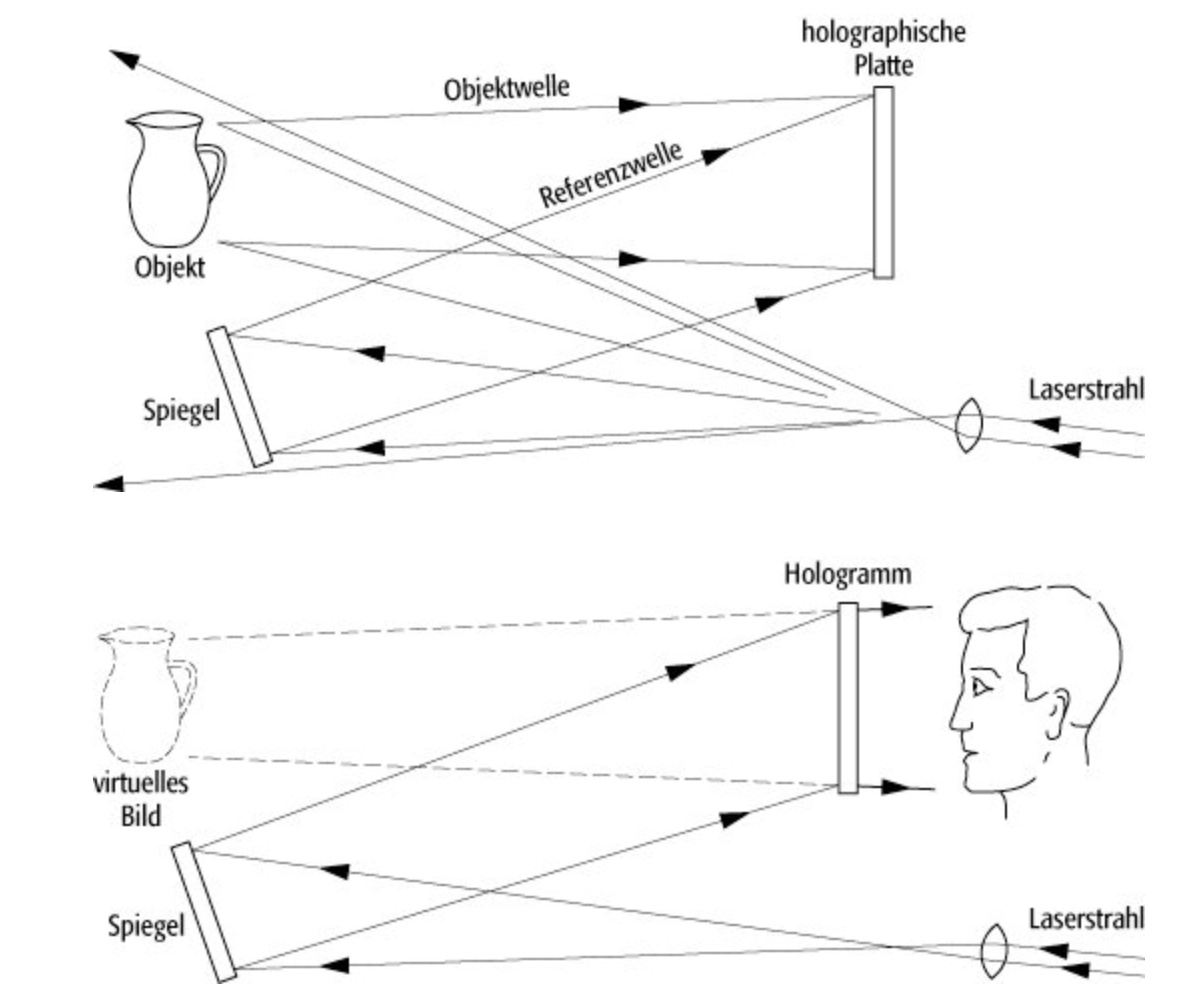
\includegraphics[scale=0.5]{Bilder/FzV/Holographie.png}
    \caption{Obere Abbildung: Schematischer Aufbau einer Aufnahme eines Hologramm. \\
    Untere Abbildung: Schematischer Aufbau einer Rekonstruktion eines Hologramm.}
\end{figure}
